\subsection{Mittellinie}
\label{ssec:fahrspurerkennung:riverflow:mittellinie}
Ähnlich wie im Kapitel~\ref{sec:maskenbau} beschrieben findet dieser Ansatz die zur Mittellinie zugehörigen Elemente, ohne auf richtig definierte \gls{acr:roi} angewiesen zu sein. Ausgangspunkt ist ebenfalls wieder das binarisierte Bild, auf das die \gls{glos:matlab}-Funktion \emph{regionprops} angewendet wird. Diese bereits verfügbare Funktion findet als Alternative zum in ~\ref{sec:maskenbau} erwähnten \glqq Ringfilter\grqq{} alle zusammenhängende Pixelgruppen und extrahiert zusätzlich eine Vielzahl derer Eigenschaften, wie Länge, Breite, Orientierung und Mittelpunkt. Da wie in Punkt~\ref{item:riverflow:rule:dashedline} bereits erwähnt die mittlere Fahrbahnmarkierung genau spezifiziert ist, werden so alle potentiellen Mittellinienstriche vorgemerkt. Diese Vorgehensweise funktioniert allerdings nur dann stabil, wenn die Güte des binarisierten Bildes gut genug ist, sodass Striche \gls{acr:zb} nicht unterbrochen sind. Trotz der guten Qualität des Bildes kommt es vor, dass falsche Bildteile als Mittellinienelemente erkannt und vorgemerkt werden. Deswegen stellen wir durch eine Verifizierung sicher, dass möglichst keine falschen Punkte in die Weltkarte, welche später zur Regelung des Autos genutzt wird, eingetragen werden. Schon an der großen Vier-Seiten-Kreuzung kommt es sonst zum Problem, dass darüber hinaus Mittellinienstriche der kreuzenden Straße erkannt werden. Auch wenn diese zur mittleren Linie gehören, sollen sie hier auf Grund des derzeitigen Regelungskonzepts noch nicht in die Karte aufgenommen werden. 
% Das ist freilich nicht falsch, aber für das aktuelle Regelungskonzept auch nicht zielführend. 

\paragraph{Verifikation}

Die Prozedur der Verifizierung verläuft nach einem vergleichbaren Prinzip wie der in~\ref{ssec:fahrspurerkennung:riverflow:randlinie} beschriebene Riverflow-Algorithmus. Dabei wird davon ausgegangen, dass sich das Fahrzeug größtenteils in der Fahrspur befindet, sodass mindestens ein Mittellinienstrich unweit vor dem Auto positioniert ist. Initial wird ein Suchfenster erstellt, welches in der Höhe den reichlichen Abstand zwischen den Mittelpunkten zweier benachbarter Mittelstreifen annimmt. Das erste sich in diesem Bereich aufhaltende Objekt wird dann als verifiziert angesehen, wenn seine Orientierung nicht übermäßig von der des Fahrzeugs abweicht. Ausgehend von diesem Punkt \glqq hangelt\grqq{} sich der Verifikations-Algorithmus von Strich zu Strich, indem er eine neue \gls{acr:roi} (ein neues Suchfenster) aufstellt. Da zu jedem (verifizierten) Punkt seine Orientierung bekannt ist, wird der nächste Mittellinienpunkt in dieser Richtung im ebenfalls bekannten Abstand zwischen zwei Punkten vermutet und dort der Mittelpunkt des neuen Suchfensters definiert. Dieses Schema wiederholt sich, bis entweder der Bildrand erreicht ist, keine Punkte im Suchfenster liegen, oder sich die Orientierung von einem zum nächsten Strich zu stark geändert hat.

Das gleiche Vorgehen wird zudem wahlweise vom ersten Punkt hinter dem Fahrzeug ausgehend wiederholt, sodass auch schon passierte Mittellinienpunkte, welche \gls{acr:zb} bei einem zukünftigen Überholvorgang benötigt werden könnten, verifiziert sind.

\begin{figure}[H]
	\centering
	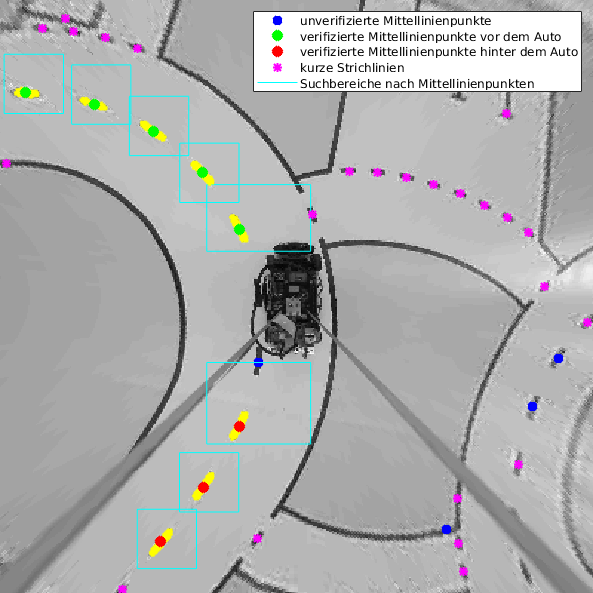
\includegraphics[width=0.9\textwidth]{fahrspurerkennung_riverflow_regionprops.png}
	\caption{Detektion von Punktgruppen mit bestimmten Eigenschaften mithilfe der \emph{regionprops}-Funktion}
	\label{fig:riverflow:mittellinie:regionprops}
\end{figure}

In \gls{acr:abb}~\ref{fig:riverflow:mittellinie:regionprops} sehen wir das Resultat der Mittellinien-/Stricherkennung. Im gleichen Zug wird die \emph{regionprops}-Funktion auch zur Randstricherkennung bei Kreuzungen genutzt. Diese Informationen werden im Riverflow-Algorithmus verwendet, welcher im nun folgenden Abschnitt beschrieben ist.